\documentclass[a4paper,twoside,10pt]{article}
%\usepackage[brazil]{babel}
%\usepackage[latin1]{inputenc}
\usepackage{multicol} % double column
\usepackage{graphicx}
\usepackage{amsmath}
\usepackage{mathptmx}
\usepackage{hyperref}% put email of author
\usepackage{amsthm}
\usepackage{amsfonts}
\usepackage{amssymb}
\usepackage[hmarginratio=1:1,top=32mm,columnsep=20pt]{geometry} % Document margins
%\usepackage{authblk}
%%%%%%%%%%%%%%%%%%%%%%%%%%%%%%%%%%%%%%%%%%%%%%%%%%%%%%%%%%%%%%%%%%%%%%%%%%%%%%%%%%%%%%%%%%%%%%%%%%%%%%%%%%%%
\usepackage{abstract} % Allows abstract customization
\renewcommand{\abstractnamefont}{\normalfont\bfseries} % Set the "Abstract" text to bold
\renewcommand{\abstracttextfont}{\normalfont\small\itshape} % Set the abstract itself to small italic text
%%%%%%%%%%%%%%%%%%%%%%%%%%%%%%%%%%%%%%%%%%%%%%%%%%%%%%%%%%%%%%%%%%%%%%%%%%%%%%%%%%%%%%%%%%%%%%%%%%%%%%%%%%%%
\usepackage{fancyhdr}
\pagestyle{fancy}
%%%%%%%%%%%%%%%%%%%%%%%%%%%%%%%%%%%%%
\lhead{}%Cabe�alho vazio � esquerda
\rhead{{\LARGE Blucher}} %Cabe�alho � direita
\chead{\bfseries Blucher Proceedings \\ VII Encontro Cient\'\i fico de F\'\i sica Aplicada} %Cabe�alho ao centro

\makeatletter
\newenvironment{tablehere}
  {\def\@captype{table}}
  {}

\newenvironment{figurehere}
  {\def\@captype{figure}}
  {}
\makeatother

%
%
%
%%%%%%%%%%%%%%%%%%%%%%%%%%%%%%%%%%%%%%%%%% Title of article%%%%%%%%%%%%%%%%%%%%%%%%%%%%%%%%%%%%%%%%%
%%%%%%%%%%%%%%%%%%%%%%%%%%%%%%%%%%%%%%%%%%%%%%%%%%%%%%%%%%%%%%%%%%%%%%%%%%%%%%%%%%%%%%%%%%%%%%%%%%%%
%
%
\title{Supernovae Observational Cosmology using GPU High Performance Computing}

%%%%%%%%%%%%%%%%%%%%%%%%%%%%%%%%%%%%%%%%%% Authtor name %%%%%%%%%%%%%%%%%%%%%%%%%%%%%%%%%%%%%%%%%%%%%%%%
%
%
\author{%\large
Colistete Jr., R. \\ % First Author
\small Departamento de Qu\'\i mica e F\'\i sica, Universidade Federal do Esp\'\i rito Santo, Alegre, ES, Brazil \\ % Institution adress
\small \href{mailto:roberto.colistete@ufes.br}{roberto.colistete@ufes.br}\\ % E-mail address
Giostri, R. \\ % SecondAuthor
\small Departamento de Qu\'\i mica e F\'\i sica, Universidade Federal do Esp\'\i rito Santo, Alegre, ES, Brazil \\ % Institution adress
\small \href{mailto:ramon.campos@ufes.br}{ramon.campos@ufes.br} % E-mail address
\vspace{-5mm}
}

\date{~~~}
%%%%%%%%%%%%%%%%%%%%%%%%%%%%%%%%%%%%%%%%%%%%%%%%%%%%%%%%%%%%%%%%%%%%%%%%%%%%%%%%%%%%%%%%%%%
\begin{document}

\maketitle % Insert title

\thispagestyle{fancy} % All pages have headers and footers
%----------------------------------------------------------------------------------------
%	ABSTRACT
%----------------------------------------------------------------------------------------
\begin{abstract}
\noindent We performed computing calculations of SNe Ia (type Ia supernova) in observational cosmology using CPU (Central Processing Unit) and GPU/CUDA (Graphics Processing Unit/Compute Unified Device Architecture) in 7 different programming methods : CUDA called from C/C++, Python with CUDA (PyCUDA), Wolfram Mathematica with CUDA, C/C++, pure Python, Python with NumPy and Wolfram Mathematica calculated in CPU. With CUDA, we obtained speedup of approximately 3 to 7 hundred times with respect to CPU when performing calculations of the SNe Ia distance modulus $(\mu_0)$. So we confirmed that CUDA (Compute Unified Device Architecture) is an excellent choice for GPU High Performance Computing (HPC) architecture applied to observational cosmology calculations.\\

Keywords: observational cosmology, high performance computing, CUDA  
\end{abstract}

%%%%%%%%%%%%%%%%%%%%%%%%%%%%%%%%%%%%%%%%%%%%%%%%%%%%%%%%%%%%%%%%%%%%%%%%%                                            
\begin{multicols}{2} % Two-column layout throughout the main article text
%%%%%%%%%%%%%%%%%%%%%%%%%%%%%%%%%%%%%%%%%%%%%%%%%%%%%%%%%%%%%%%%%%%%%%%%%%

\section{Introduction}
Advances in computational techniques have allowed to explore issues related to science and technology that were previously unimaginable, one of them is the development of High Performance Computing (HPC) based on parallel computing using GPU (Graphics Processing Unit).
              
We targeted the problem of calculating the distance modulus $(\mu_0)$ for type Ia supernovae (SNe Ia), used in observational cosmology to estimate the theoretical cosmological models. Those models can sometimes have a parameter space with many dimensions and Bayesian statistics need a large number of points in the parameter space to marginalize parameters and compare models.

For the case of flat standard model of cosmology \cite{wang} there are $N=3$ free parameters. Under these conditions the calculation is performed about $10^3$ times for each supernova. But for supported models with $N$ dimensions, it can vary between $10^N$ to $10^{2N}$. Also worth remembering is that today the supernovae catalogs are of the order of a thousand supernovae and the estimate is that with new experiments it will have hundreds of thousands of SNe Ia in a few years \cite{weinberg}. Given the values shown we have a very intensive computational problem, so those SNe Ia calculations are a good application for HPC with GPU.                            
                            
In this context, we performed the calculation of the distance modulus $(\mu_0)$ on CPU with no parallelism by using the programming languages C/C++, pure Python, Python with Numpy and Wolfram Mathematica \cite{mathematica}. Then we used GPU and CUDA (Compute Unified Device Architecture) \cite{cuda}, we calculated $\mu_0$ with CUDA (called from C/C++), PyCUDA \cite{pycuda} (Python with CUDA) and Wolfram Mathematica with CUDA. We compared the advantages and disadvantages of these approaches.

         
\section{Type Ia supernova observational cosmology}

A supernova is one of the possible final stages of a star, there are several types of supernovae \cite{filippenko} and we give particular attention to the type Ia supernovae (SNe Ia). The SNe Ia are standardizable candles and this feature was essential to prove that the universe expands with acceleration in 1998/1999 \cite{riess,permutter}, this pioneering work have won the Nobel prize in 2011.

Calculation of the theoretical distance modulus $\mu_0$ is a central part of SNe Ia observational cosmology, as it is the amount statistically compared with the astronomical observable:
{\small
\begin{equation}
 \mu_0(z,\Theta)=25+5\,log_{10}\left( \frac{(1+z)c}{H_0}\int_{0}^{z}\frac{1}{h(z',\Theta)}dz' \right)
\end{equation}}

For flat cosmological models the changes are in the denominator of integrand, for non flat models, more significant changes are necessary \cite{drell}.          


\section{Performance of $\mu_0$ calculations in CPU and GPU}

The calculation of the theoretical distance modulus $\mu_0$ was performed on CPU and GPU using single precision (SP) and double precision (DP). We obtained the speedup of GPU calculations with respect to C/C++ running on 1 CPU core (figures \ref{figSP}-\ref{figDP}), and compared the calculation time in 7 different programming methods (table \ref{tableDP}). 

The configuration in terms of hardware and software : workstation with Intel Core i7 4770K (3.5-3.9 GHz, 8MB cache, 4 cores, 8 threads), 16GB RAM, GeForce GTX Titan (2,688 cores, 6GB GDDR5 RAM), Ubuntu 14.04.2 64 bits, Linux kernel 3.16.0, gcc 4.8.4, Python 2.7.6, NumPy 1.8.2, CUDA 7.0-28, PyCUDA v2015.1, Mathematica 10.1.

\begin{figurehere}
\centering
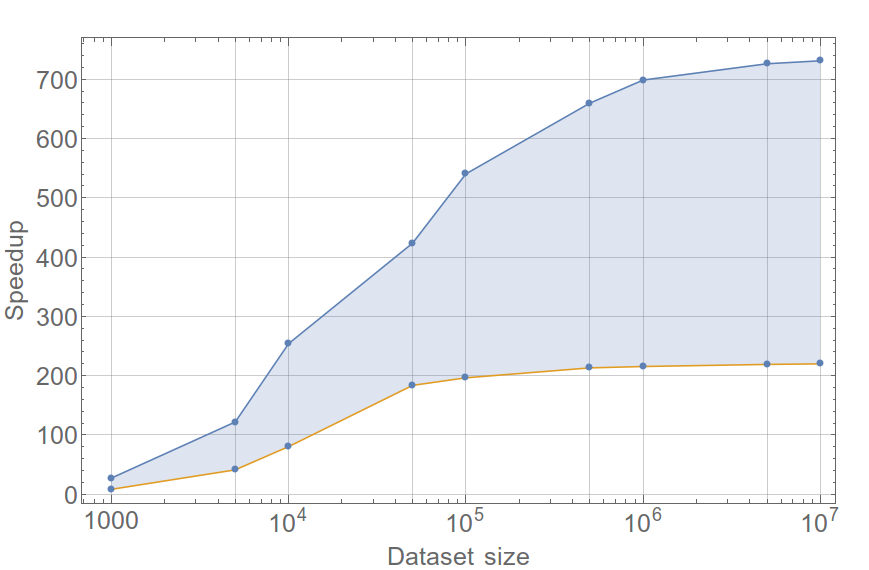
\includegraphics[scale=0.23]{Grafico_ganho_x_num_SP.png}
\caption{{\small Speedup with respect C/C++ (in 1 CPU core) vs. dataset size (number of supernovae) in SP (single precision)). C/C++/CUDA in blue, PyCUDA in orange. Wolfram Mathematica 10 using CUDA is not shown because it doesn't work in SP.}}
\label{figSP}
\end{figurehere}
\begin{figurehere}
\centering
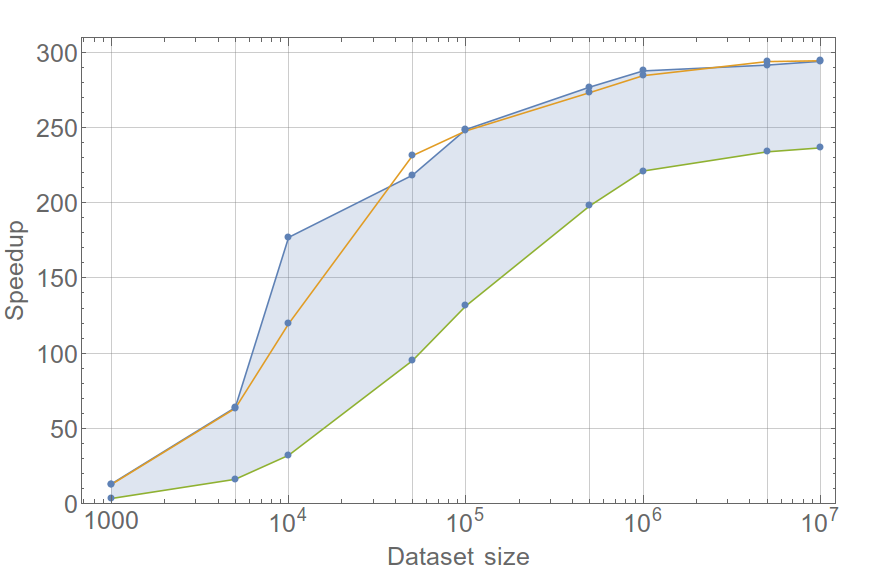
\includegraphics[scale=0.23]{Grafico_ganho_x_num_DP.png}
\caption{{\small Speedup with respect C/C++ (in 1 CPU core) vs. dataset size (number of supernovae) in DP (double precision). C/C++/CUDA in blue, PyCUDA in orange, Wolfram Mathematica 10 using CUDA in green.}}
\label{figDP}
\end{figurehere}

\begin{tablehere}
\begin{center}
\caption{{\small $\mu_0$ DP (double precision) calculation time in seconds (s) for $10^5$ SNe Ia. CUDA : C/C++/CUDA. WMC : Wolfram Mathematica 10 using CUDA. Python : pure Python. NumPy : Python with NumPy. WM : Wolfram Mathematica 10 using CPU. }}
\label{tableDP}
\begin{tabular}{ccc}
\hline
Method & Total time (s) & Kernel time (s) \\
\hline
CUDA & 0.002941 & 0.002576 \\
PyCUDA & 0.002952 & 0.002450 \\
WMC & 0.006366 & 0.003632 \\
C/C++ & 0.7327 & --- \\
Python & 46.13 & --- \\
NumPy & 1.499 & --- \\
WM & 2.634 & --- \\
\hline
\end{tabular}
\end{center}

\end{tablehere}

In SP (single precision), C/C++/CUDA is 1-2 times faster than PyCUDA because PyCUDA has overhead in dealing with SP data. While Wolfram Mathematica versions 9/10 don't calculate at all when running kernels in SP.
               
In DP (double precision), PyCUDA is approximately as fast as C/C++/CUDA. Both are faster than Wolfram Mathematica with CUDA, which is not efficient in CPU-GPU communication.

Performance wise in SP, C/C++/CUDA speedup w.r.t. C/C++ (CPU using 1 core) is up to 730 times. PyCUDA speedup w.r.t. C/C++ is up 220 times, w.r.t. Python/NumPy is up to 450 times. So C/C++/CUDA is 1-2 times faster than PyCUDA in SP.
               
In DP, PyCUDA is approximately as fast as C/C++/CUDA : C/C++/CUDA speedup w.r.t. C/C++ is up to 294 times. PyCUDA speedup w.r.t. C/C++ is up 294 times, w.r.t. Python/NumPy is up to 601 times. Wolfram Mathematica with CUDA speedup w.r.t. C/C++ is up to 237, w.r.t. to Mathematica (using CPU) is up to 852 times.


\section{Conclusion}

The use of GPU with CUDA applied to calculations of the SNe Ia distance modulus $(\mu_0)$ yields an impressive speedup of approximately 3 to 7 hundred times with respect to CPU. 

CUDA is usually called from C/C++, but there is also PyCUDA which let us use CUDA from Python, making HPC with GPU easier with respect to C/C++ with CUDA, while being robust and giving good performance.
               
Wolfram Mathematica, which has an interpreted and high level language, can also call CUDA since version 8, so it was compared here.

Both PyCUDA and Wolfram Mathematica with CUDA use interpreted and higher level programming languagens so they are easier to program (resulting less code and less time to develop) than pure C/C++/CUDA. They also allow metaprogramming (computer programs creating computer programs).
			                
So PyCUDA compares very well, being : as fast as C/C++/CUDA in double precision; faster and more robust than Wolfram Mathematica with CUDA; hundreds times faster than C/C++, pure Python, Python with NumPy, and Wolfram Mathematica calculated in CPU.
               
So we concluded that HPC with GPU/CUDA is an excellent choice for SNe Ia observational cosmology calculations. And PyCUDA is a very attractive and competitive choice for CUDA programming.


\begin{thebibliography}{99}

\bibitem{wang} Wang, Y., et al. Dark Energy. Weinheim, Germany, Wiley, 2010.

\bibitem{weinberg} Weinberg, D. H., et al. Physics Reports, v. 530, Issue 2, p. 87-256, 2013.

\bibitem{mathematica}  Wolfram, S. Mathematica: A System for Doing Mathematics by Computer, 2nd edition. Redwood City, Addison-Wesley, 1991.

\bibitem{cuda} Nickolls, J., et al. ACM Queue, v. 6, n. 2, p. 40-53, March/April 2008, 

\bibitem{pycuda} Kl�ckner, A., et al. Parallel Computing, v. 38, issue 3, p. 157-174, March 2012.

\bibitem{filippenko} Filippenko, A. V. Annu. Rev. Astron. Astrophys, v. 35, p. 309-355, 1997.

\bibitem{riess} Riess, A. G., et al. Astron. J., v. 116, p. 1009-1038, 1998.

\bibitem{permutter} Permutter, S., et al. Astrophys. J., v. 517, p. 565-586, 1999.

\bibitem{drell} Drell, P. S., et al. Astrophys. J., v. 530, p. 593-617, 2000.

\end{thebibliography} 
\end{multicols}
\end{document}
